%%%%%%%%%%%%%%%%%%%%%%%%%%%%%%%%%%%%%%%%%%%%%%%%%%%%%%%%%%%%%%%%%%%%%
%%                                                                 %%
%% Please do not use \input{...} to include other tex files.       %%
%% Submit your LaTeX manuscript as one .tex document.              %%
%%                                                                 %%
%% All additional figures and files should be attached             %%
%% separately and not embedded in the \TeX\ document itself.       %%
%%                                                                 %%
%%%%%%%%%%%%%%%%%%%%%%%%%%%%%%%%%%%%%%%%%%%%%%%%%%%%%%%%%%%%%%%%%%%%%

%%\documentclass[referee,sn-basic]{sn-jnl}% referee option is meant for double line spacing

%%=======================================================%%
%% to print line numbers in the margin use lineno option %%
%%=======================================================%%

%%\documentclass[lineno,sn-basic]{sn-jnl}% Basic Springer Nature Reference Style/Chemistry Reference Style

%%======================================================%%
%% to compile with pdflatex/xelatex use pdflatex option %%
%%======================================================%%

%%\documentclass[pdflatex,sn-basic]{sn-jnl}% Basic Springer Nature Reference Style/Chemistry Reference Style

%%\documentclass[sn-basic]{sn-jnl}% Basic Springer Nature Reference Style/Chemistry Reference Style
\documentclass[pdflatex,sn-mathphys]{sn-jnl}% Math and Physical Sciences Reference Style
\usepackage{array}
%%\documentclass[sn-aps]{sn-jnl}% American Physical Society (APS) Reference Style
%%\documentclass[sn-vancouver]{sn-jnl}% Vancouver Reference Style
%%\documentclass[sn-apa]{sn-jnl}% APA Reference Style
%%\documentclass[sn-chicago]{sn-jnl}% Chicago-based Humanities Reference Style
%%\documentclass[sn-standardnature]{sn-jnl}% Standard Nature Portfolio Reference Style
%%\documentclass[default]{sn-jnl}% Default
%%\documentclass[default,iicol]{sn-jnl}% Default with double column layout

%%%% Standard Packages
%%<additional latex packages if required can be included here>
%%%%

%%%%%=============================================================================%%%%
%%%%  Remarks: This template is provided to aid authors with the preparation
%%%%  of original research articles intended for submission to journals published 
%%%%  by Springer Nature. The guidance has been prepared in partnership with 
%%%%  production teams to conform to Springer Nature technical requirements. 
%%%%  Editorial and presentation requirements differ among journal portfolios and 
%%%%  research disciplines. You may find sections in this template are irrelevant 
%%%%  to your work and are empowered to omit any such section if allowed by the 
%%%%  journal you intend to submit to. The submission guidelines and policies 
%%%%  of the journal take precedence. A detailed User Manual is available in the 
%%%%  template package for technical guidance.
%%%%%=============================================================================%%%%

\jyear{2022}%

%% as per the requirement new theorem styles can be included as shown below
\theoremstyle{thmstyleone}%
\newtheorem{theorem}{Theorem}%  meant for continuous numbers
%%\newtheorem{theorem}{Theorem}[section]% meant for sectionwise numbers
%% optional argument [theorem] produces theorem numbering sequence instead of independent numbers for Proposition
\newtheorem{proposition}[theorem]{Proposition}% 
%%\newtheorem{proposition}{Proposition}% to get separate numbers for theorem and proposition etc.

\theoremstyle{thmstyletwo}%
\newtheorem{example}{Example}%
\newtheorem{remark}{Remark}%

\theoremstyle{thmstylethree}%
\newtheorem{definition}{Definition}%

\raggedbottom
%%\unnumbered% uncomment this for unnumbered level heads

\begin{document}

\title[Enzyme Kinetics and Energetics]{Lab Report on Enzyme Activity and Kinetics}

%%=============================================================%%
%% Prefix	-> \pfx{Dr}
%% GivenName	-> \fnm{Joergen W.}
%% Particle	-> \spfx{van der} -> surname prefix
%% FamilyName	-> \sur{Ploeg}
%% Suffix	-> \sfx{IV}
%% NatureName	-> \tanm{Poet Laureate} -> Title after name
%% Degrees	-> \dgr{MSc, PhD}
%% \author*[1,2]{\pfx{Dr} \fnm{Joergen W.} \spfx{van der} \sur{Ploeg} \sfx{IV} \tanm{Poet Laureate} 
%%                 \dgr{MSc, PhD}}\email{iauthor@gmail.com}
%%=============================================================%%

\author*[1,2]{\fnm{Harsh} \sur{Agrawal}}\email{ha1822@ic.ac.uk}

\affil*[1]{\orgdiv{Molecular Bioengineering}, \orgname{Imperial College London}}

%%==================================%%
%% sample for unstructured abstract %%
%%==================================%%

\abstract{The purpose of this set of experiments was to determine and study the activity of enzyme action under various conditions. These included pH action under different pH, temperatures, and in the presence of a competitive inhibitor.}

%%================================%%
%% Sample for structured abstract %%
%%================================%%

% \abstract{\textbf{Purpose:} The abstract serves both as a general introduction to the topic and as a brief, non-technical summary of the main results and their implications. The abstract must not include subheadings (unless expressly permitted in the journal's Instructions to Authors), equations or citations. As a guide the abstract should not exceed 200 words. Most journals do not set a hard limit however authors are advised to check the author instructions for the journal they are submitting to.
% 
% \textbf{Methods:} The abstract serves both as a general introduction to the topic and as a brief, non-technical summary of the main results and their implications. The abstract must not include subheadings (unless expressly permitted in the journal's Instructions to Authors), equations or citations. As a guide the abstract should not exceed 200 words. Most journals do not set a hard limit however authors are advised to check the author instructions for the journal they are submitting to.
% 
% \textbf{Results:} The abstract serves both as a general introduction to the topic and as a brief, non-technical summary of the main results and their implications. The abstract must not include subheadings (unless expressly permitted in the journal's Instructions to Authors), equations or citations. As a guide the abstract should not exceed 200 words. Most journals do not set a hard limit however authors are advised to check the author instructions for the journal they are submitting to.
% 
% \textbf{Conclusion:} The abstract serves both as a general introduction to the topic and as a brief, non-technical summary of the main results and their implications. The abstract must not include subheadings (unless expressly permitted in the journal's Instructions to Authors), equations or citations. As a guide the abstract should not exceed 200 words. Most journals do not set a hard limit however authors are advised to check the author instructions for the journal they are submitting to.}

% \keywords{keyword1, Keyword2, Keyword3, Keyword4}

%%\pacs[JEL Classification]{D8, H51}

%%\pacs[MSC Classification]{35A01, 65L10, 65L12, 65L20, 65L70}

\maketitle

\section{Experiment 1}\label{sec1}
\subsection{Generation of Standardization curve for p-nitrophenol}
Different serial dilutions were prepared for p-nitrophenol and the absorbances
were recorded at 410 nm to obtain the following standardization curve.
\begin{figure}[h]
  \centering
  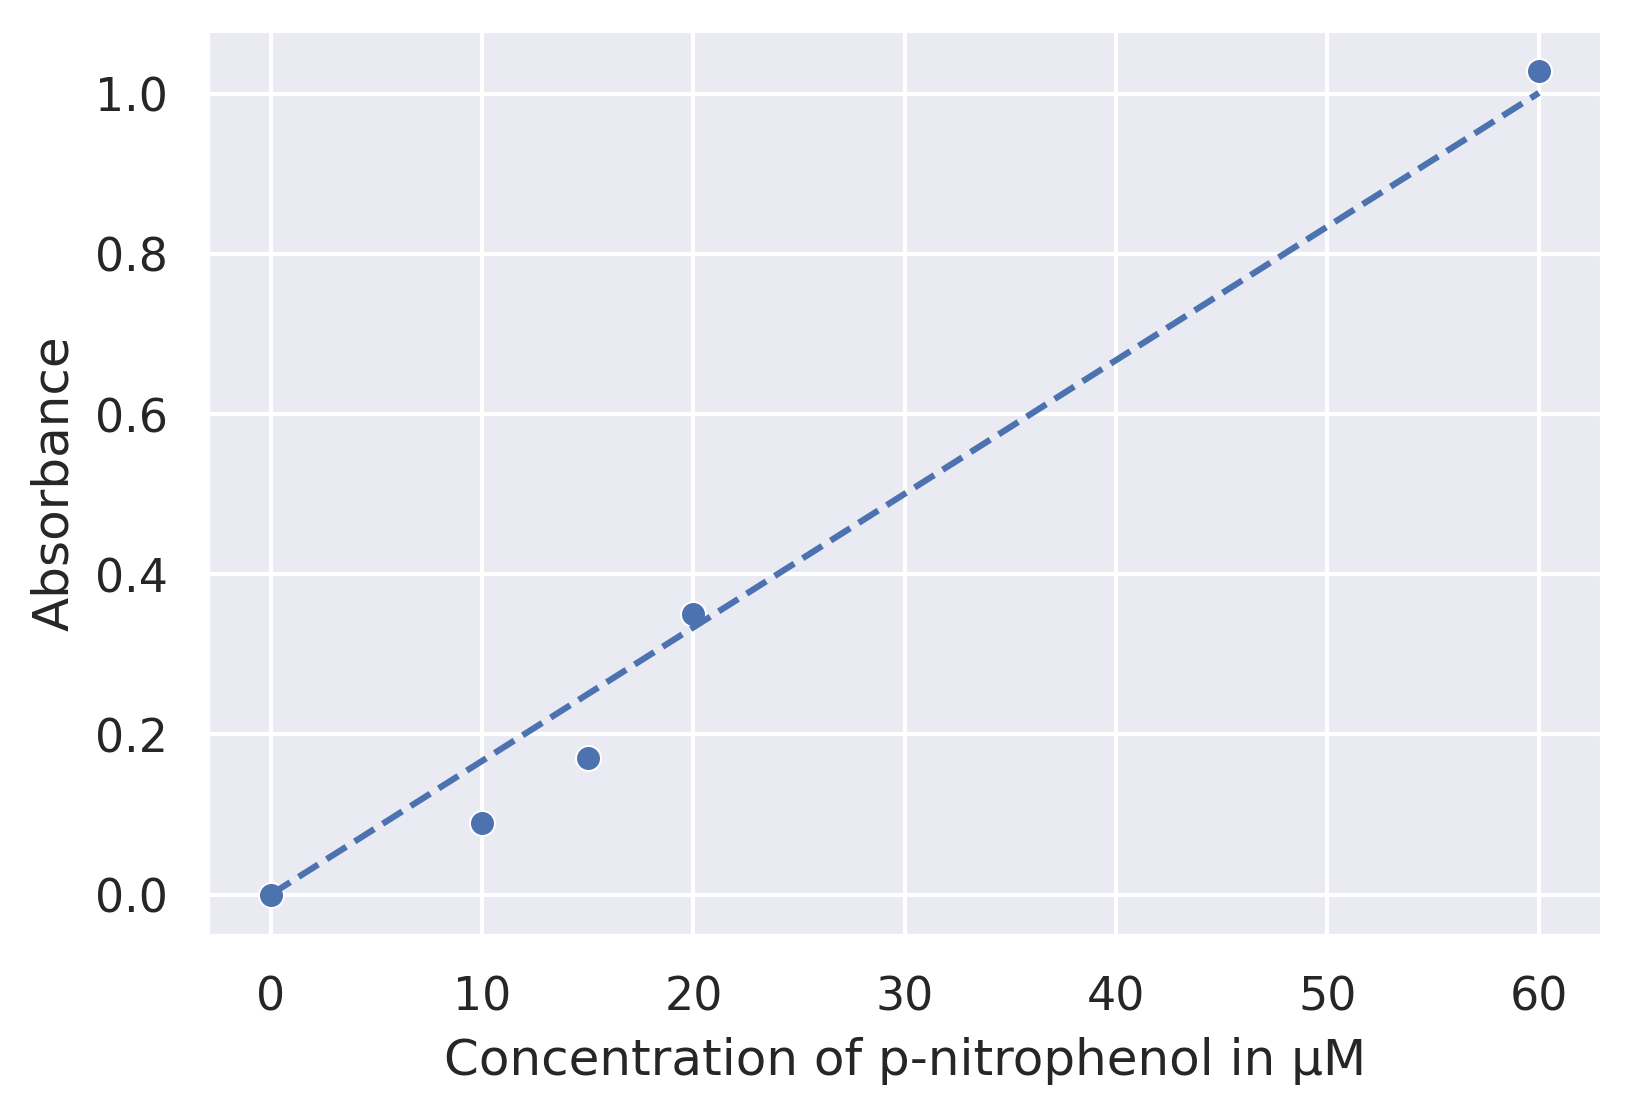
\includegraphics[width=0.6\textwidth]{photos/standardization_curve.png}
  \caption{Standardization Curve of p-nitrophenol. }\label{fig1}
\end{figure}
The line of best fit was plotted by adjusting the regression line to pass through the origin. The equation of the line plotted is:
\[y = 0.0171x + 0.00222\]
\subsection{Determination of optimum pH of phosphatase}
Citrate buffers with five different pH values (3 - 7) were added to the
different vials containing p-nitrophenyl phosphate. While keeping controls for
every pH, 1 mL of phosphatase solutions was added to each vial. After
\textbf{exactly 40 minutes}, the reactions were stopped by adding NaOH. The
absorbance was then read at 410nm and the product concentration was inferred
from the calibration curve generated above.

\begin{table}[h]
  \begin{center}
    \begin{minipage}{300pt}
      \caption{Velocity of Enzyme Activity vs pH}\label{tab1}
      \begin{tabular}{  m{4em}  m{4em} m{4.5em}  m{4.5em}  m{4.5em} m{4.5em}}
        % {@{\extracolsep{\fill}}lcccccc@{\extracolsep{\fill}}}
        \toprule
        Vial Number & pH  & Vial Type & A\textsubscript{410} (OD) & Product Conc.\footnotemark[1] ($\mu$M) & Velocity ($\mu$M/min) \\
        \midrule
        1.          & 3.0 & Test      & 0.226                     & 22.60                                  & 0.56                  \\
        2.          & 3.0 & Control   & 0.000                     & -                                      & -                     \\
        3.          & 4.0 & Test      & 0.425                     & 42.50                                  & 1.06                  \\
        4.          & 4.0 & Control   & 0.000                     & -                                      & -                     \\
        5.          & 5.0 & Test      & 0.723                     & 72.30                                  & 1.80                  \\
        6.          & 5.0 & Control   & 0.000                     & -                                      & -                     \\
        7.          & 6.0 & Test      & 0.702                     & 70.20                                  & 1.75                  \\
        8.          & 6.0 & Control   & 0.000                     & -                                      & -                     \\
        9.          & 7.0 & Test      & 0.378                     & 37.80                                  & 0.94                  \\
        10.         & 7.0 & Control   & 0.000                     & -                                      & -                     \\
        \botrule
      \end{tabular}
      \footnotetext[1]{The concentration of the product was doubled since the assay was diluted two-fold by the addition of 3mL HCl.}
    \end{minipage}
  \end{center}
\end{table}
\begin{figure}[h]
  \centering
  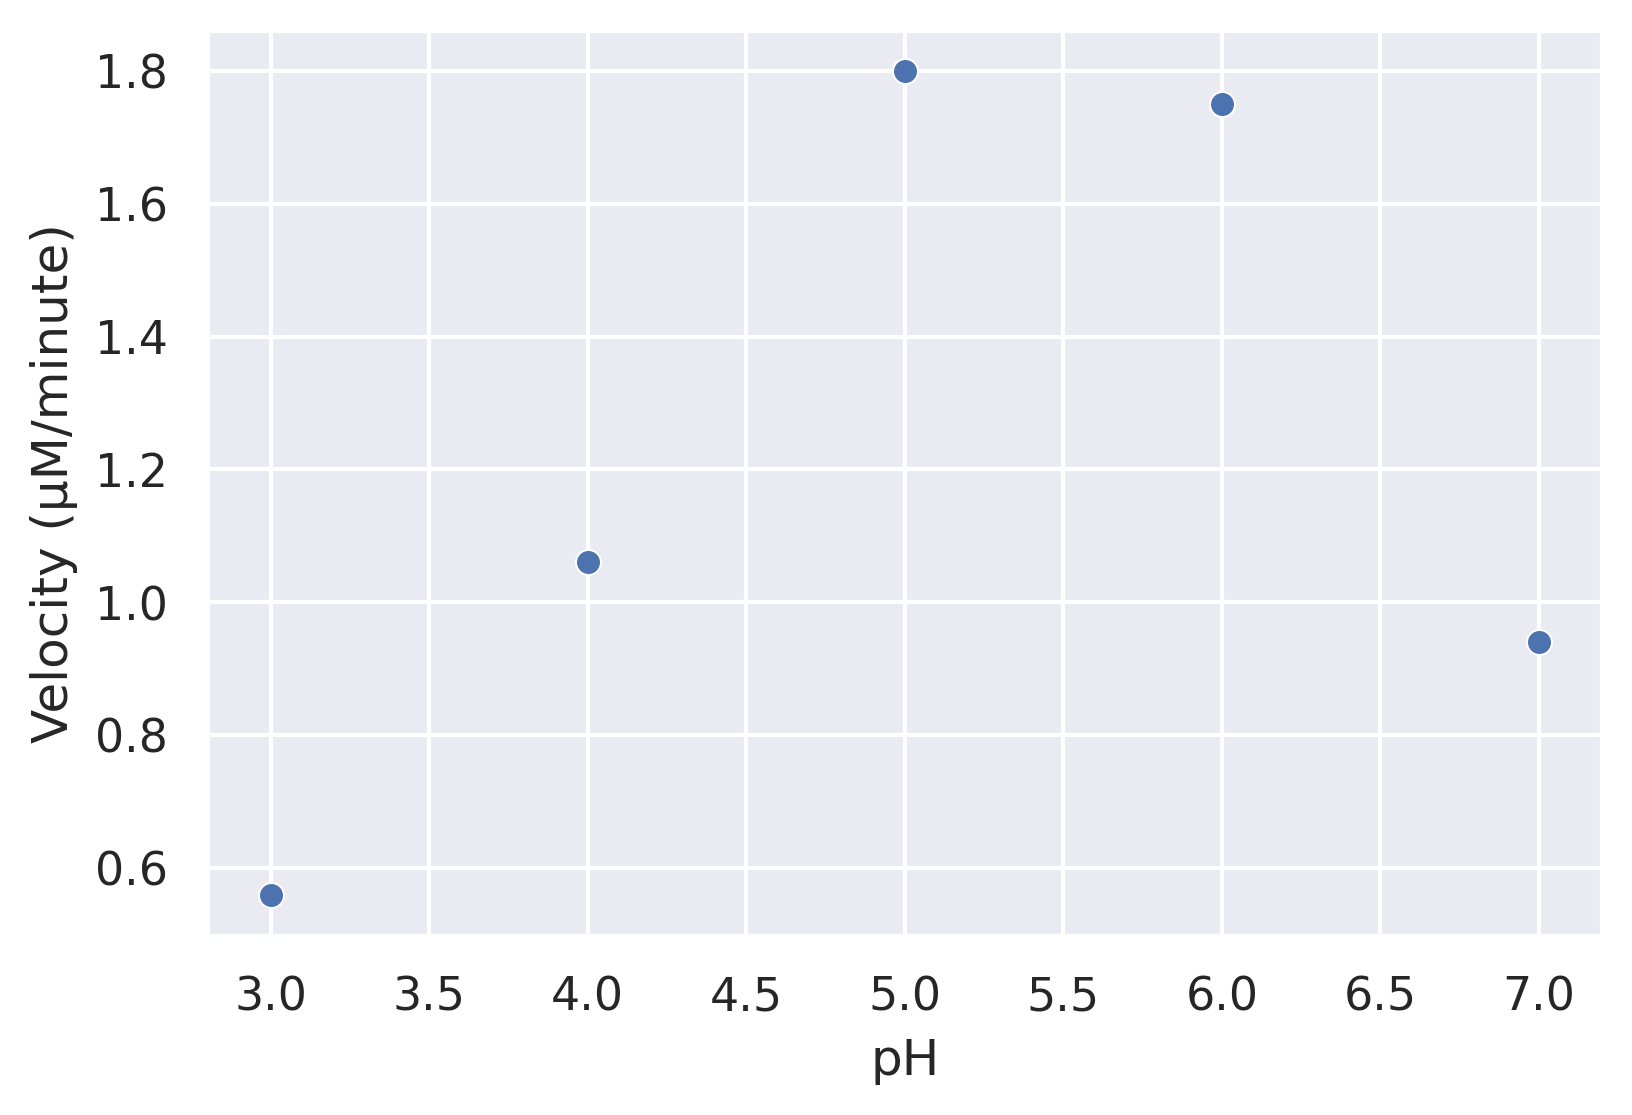
\includegraphics[width=0.6\textwidth]{photos/pH_plot.png}
  \caption{Scatterplot of the velocity of reaction ( $\mu$M of product liberated per minute) vs. pH. }\label{fig1}
\end{figure}

We can clearly observe that the velocity first increases within the increase in
pH and then falls off after pH 5.0. To determine the two principal ionizations,
the two inflection points need to be determined from the curve above. A
Gaussian distribution curve was fit on top of the curve to obtain the gaussian
function of the above graph:

\[y = 1.86201e^{-\frac{(x - 5.395395)^2}{2(1.42176)^2}}\]
The first-order differential of the function was taken and set to zero to
obtain the critical points. Followingly, a second-order derivative was taken to
infer the point of change of sign to obtain the inflection points. The
inflections points obtained were:

\[P1 = (3.97, 1.12); P2 = (6.81, 1.12)\]
Hence, these points represent the two principal ionizations. The pH at these
ionizations (x-value) are the pK_a values.

\[pK_a (1) = 3.97; pK_a (2) = 6.81\]

\subsection{Phosphate as a competitive inhibitor of phosphatase}
When phosphate is added, it competes for the binding site of acid phosphatase,
thus preventing it to bind to p-NPP. This results in an inhibition of product
formulation overall. Phosphate was used as a competitive inhibitor for a total
of five different dilutions of p-nitrophenyl phosphate - 0.0001M, 0.0004M,
0.002M, 0.004M, and 0.006M.

After exactly 26 minutes, the reactions were stopped with NaOH and the
absorbances were read. The following table summarizes the absorbance for every
vial along with the concentration and velocity inferred with the help of the
calibration curve created earlier.

\begin{table}[h]
  \begin{center}
    \begin{minipage}{300pt}
      \caption{Velocity of Enzyme Activity vs pH}\label{tab1}
      \begin{tabular}{  m{4em}  m{4em} m{4.5em}  m{4.5em}  m{4.5em} m{4.5em}}
        % {@{\extracolsep{\fill}}lcccccc@{\extracolsep{\fill}}}
        \toprule
        Vial Number & p-NPP conc. (M) & Phosphate Added & A\textsubscript{410} (OD) & Product Conc.\footnotemark[1] ($\mu$M) & Velocity ($\mu$M/min) \\
        \midrule
        1.          & 0.0001          & Yes             & 0.014                     & 1.38                                   & 0.05                  \\
        2.          & 0.0001          & No              & 0.139                     & 16.00                                  & 0.62                  \\
        3.          & 0.0001          & Yes             & 0.000                     & -                                      & -                     \\
        4.          & 0.0004          & Yes             & 0.058                     & 6.52                                   & 0.25                  \\
        5.          & 0.0004          & No              & 0.256                     & 29.68                                  & 1.14                  \\
        6.          & 0.0004          & Yes             & 0.000                     & -                                      & -                     \\
        7.          & 0.002           & Yes             & 0.176                     & 20.33                                  & 0.78                  \\
        8.          & 0.002           & No              & 0.351                     & 40.79                                  & 1.57                  \\
        9.          & 0.002           & Yes             & 0.000                     & -                                      & -                     \\
        10.         & 0.004           & Yes             & 0.249                     & 28.86                                  & 1.11                  \\
        11.         & 0.004           & No              & 0.377                     & 43.83                                  & 1.69                  \\
        12.         & 0.004           & Yes             & 0.000                     & -                                      & -                     \\
        13.         & 0.006           & Yes             & 0.180                     & 20.79                                  & 1.22                  \\
        14.         & 0.006           & No              & 0.401                     & 46.64                                  & 1.79                  \\
        15.         & 0.006           & Yes             & 0.000                     & -                                      & -                     \\
        \botrule
      \end{tabular}
      \footnotetext[1]{The concentration of the product was doubled since the assay was diluted two-fold by the addition of 3mL HCl.}
      \footnotetext[2]{Due to contamination, the reaction in vial 13 was redone. While all reactions were stopped after 26 minutes, this reaction was stopped after 17 minutes due to time constraints.}
    \end{minipage}
  \end{center}
\end{table}

\begin{figure}[h]
  \centering
  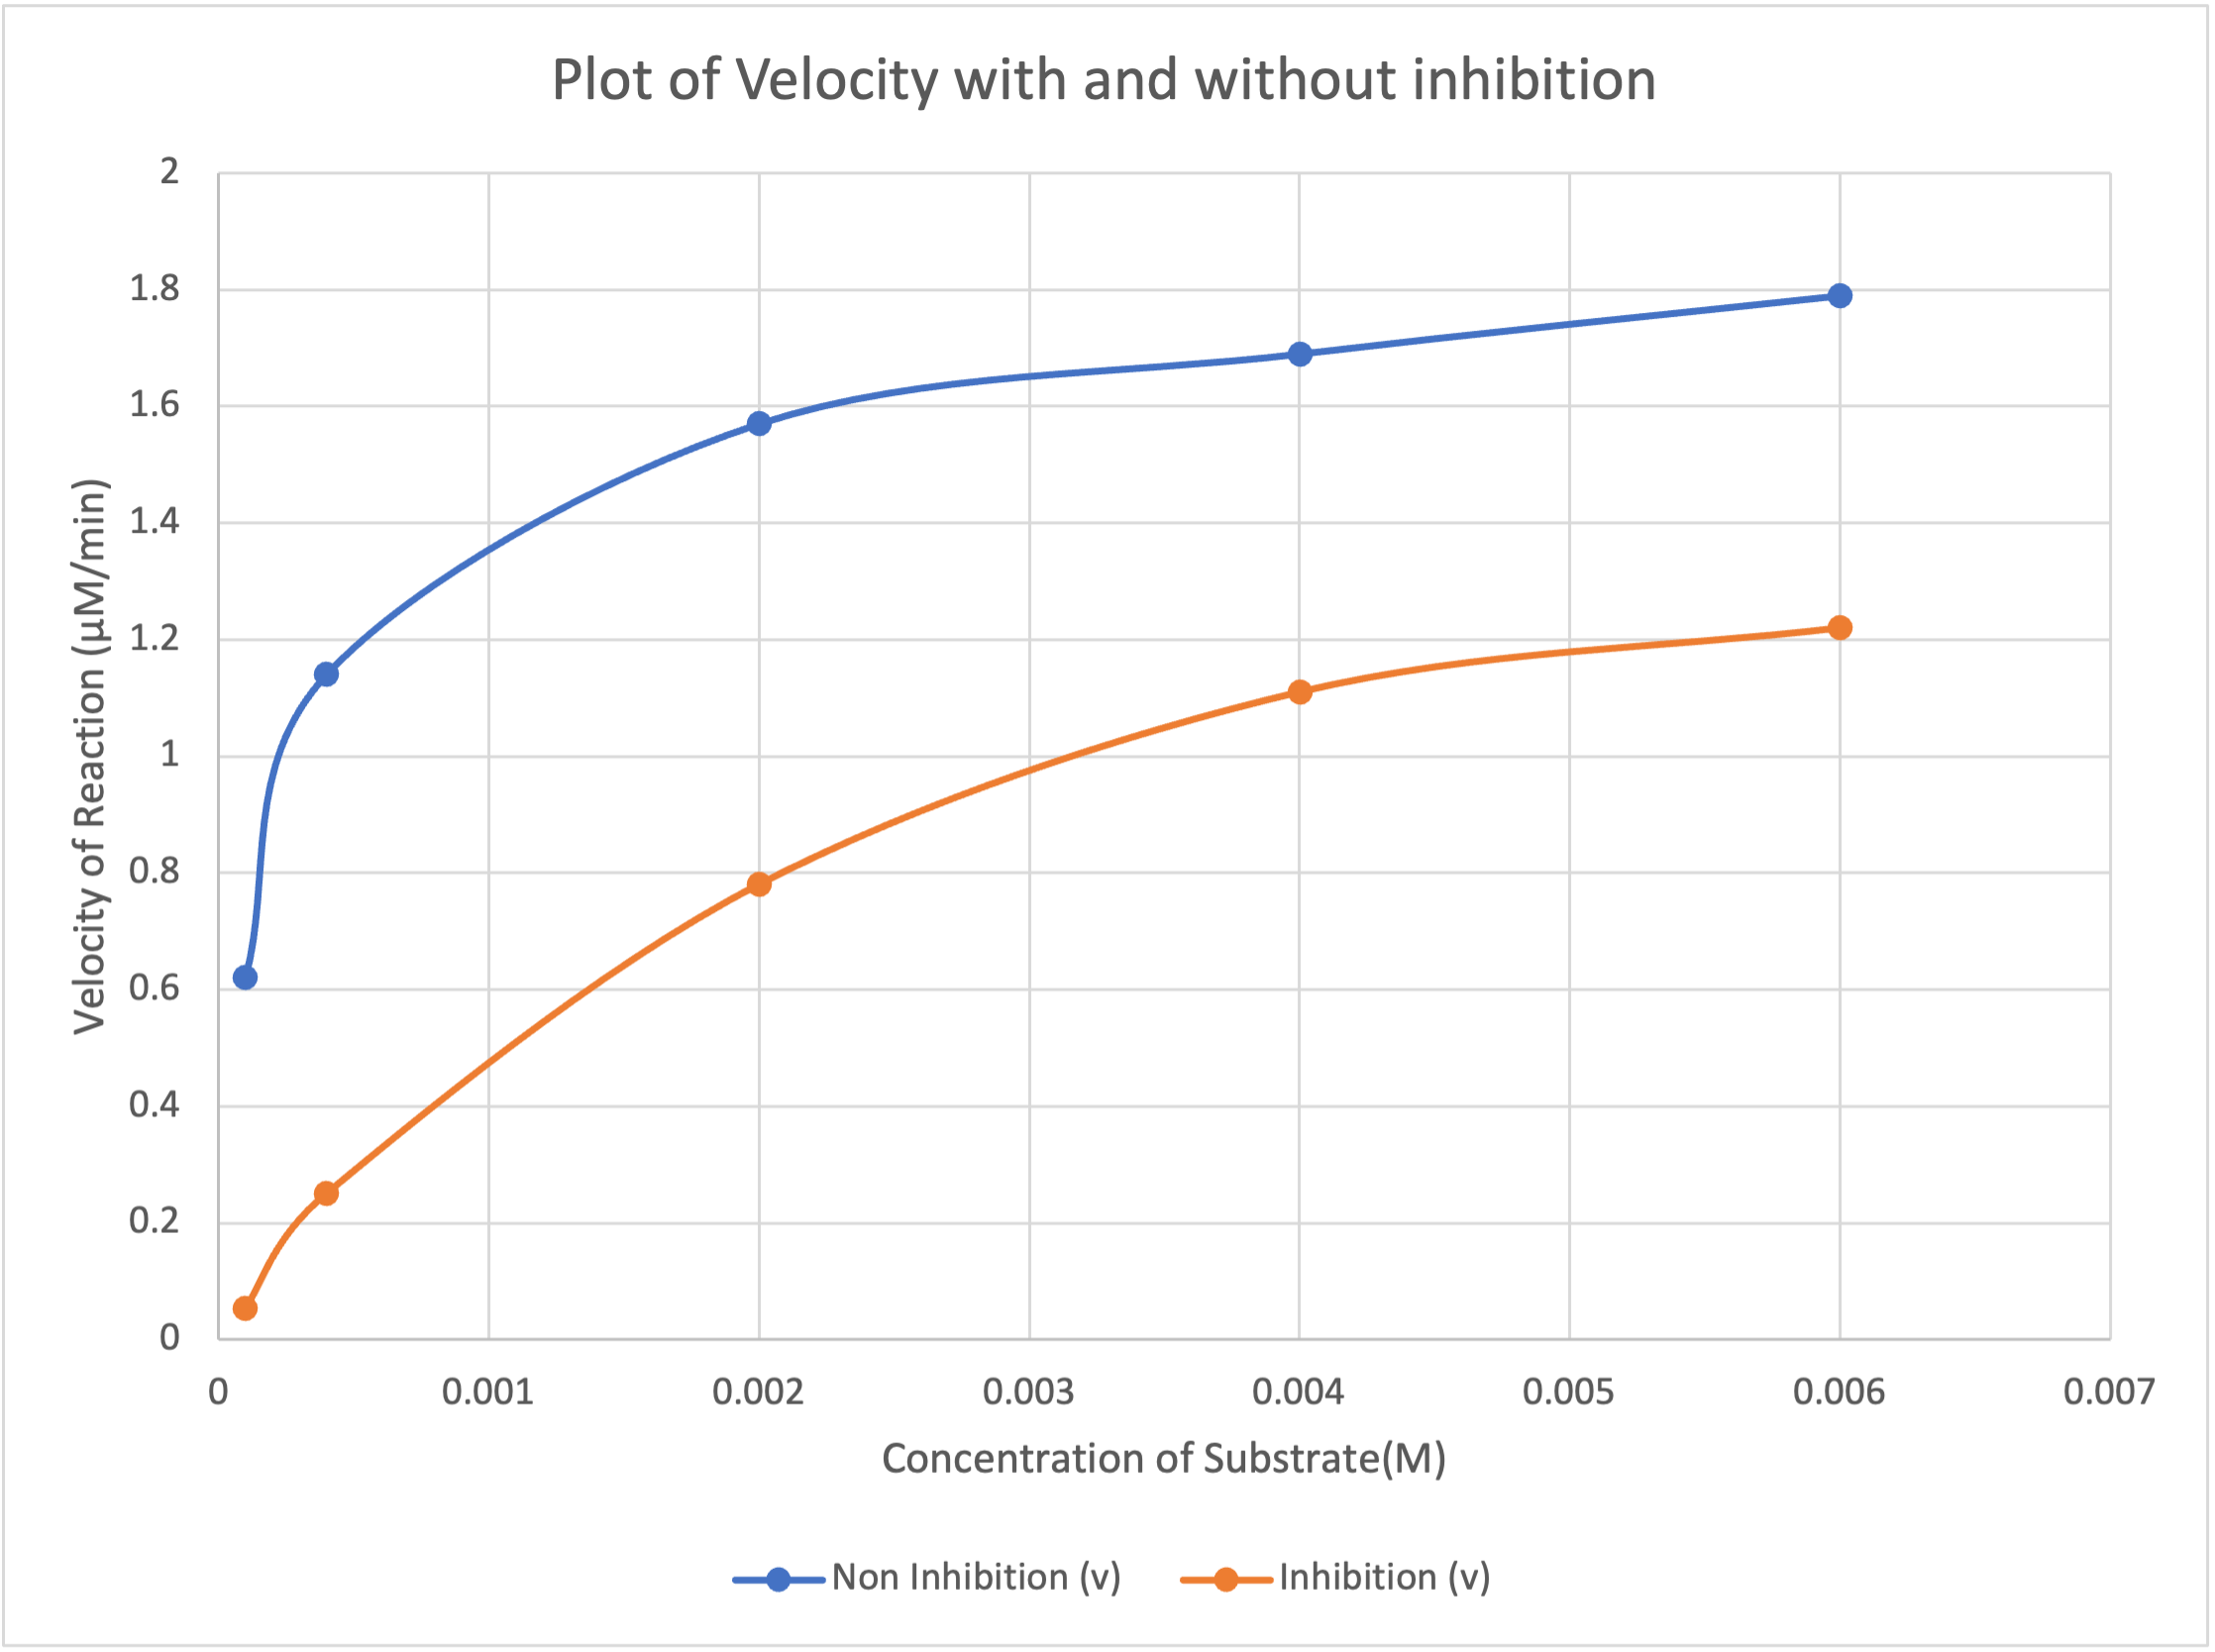
\includegraphics[width=0.6\textwidth]{photos/mm.png}
  \caption{Michaelis Menten plot of Substrate concentration (M) vs Velocity of Rection  ($\mu$M/min). }\label{fig3_1}
\end{figure}

The next step was to calculate V\textsubscript{max} and K\textsubscript{m} from
the Micheales Menten plot. A rectangular hyperbola was fit and the equations
for the two different curves (inhibition and non-inhibition) were obtained.

With competitive inhibitor $\Rightarrow$
\[y = \frac{1.725x}{0.00237 + x}\]
\[ V_{\text{max}} = 1.725\,\mu\text{M/min},  K_m = 0.00237\,\text{M}\]

Without competitive inhibitor $\Rightarrow$
\[y = \frac{1.789x}{0.000211+ x}\]

\[ V_{\text{max}} = 1.789\,\mu\text{M/min},  K_m = 0.000211\,\text{M}\]
To ensure that the above-inferred values are correct, a Lineweaver-Burk plot
was plotted using the values obtained.

\begin{figure}[h]
  \centering
  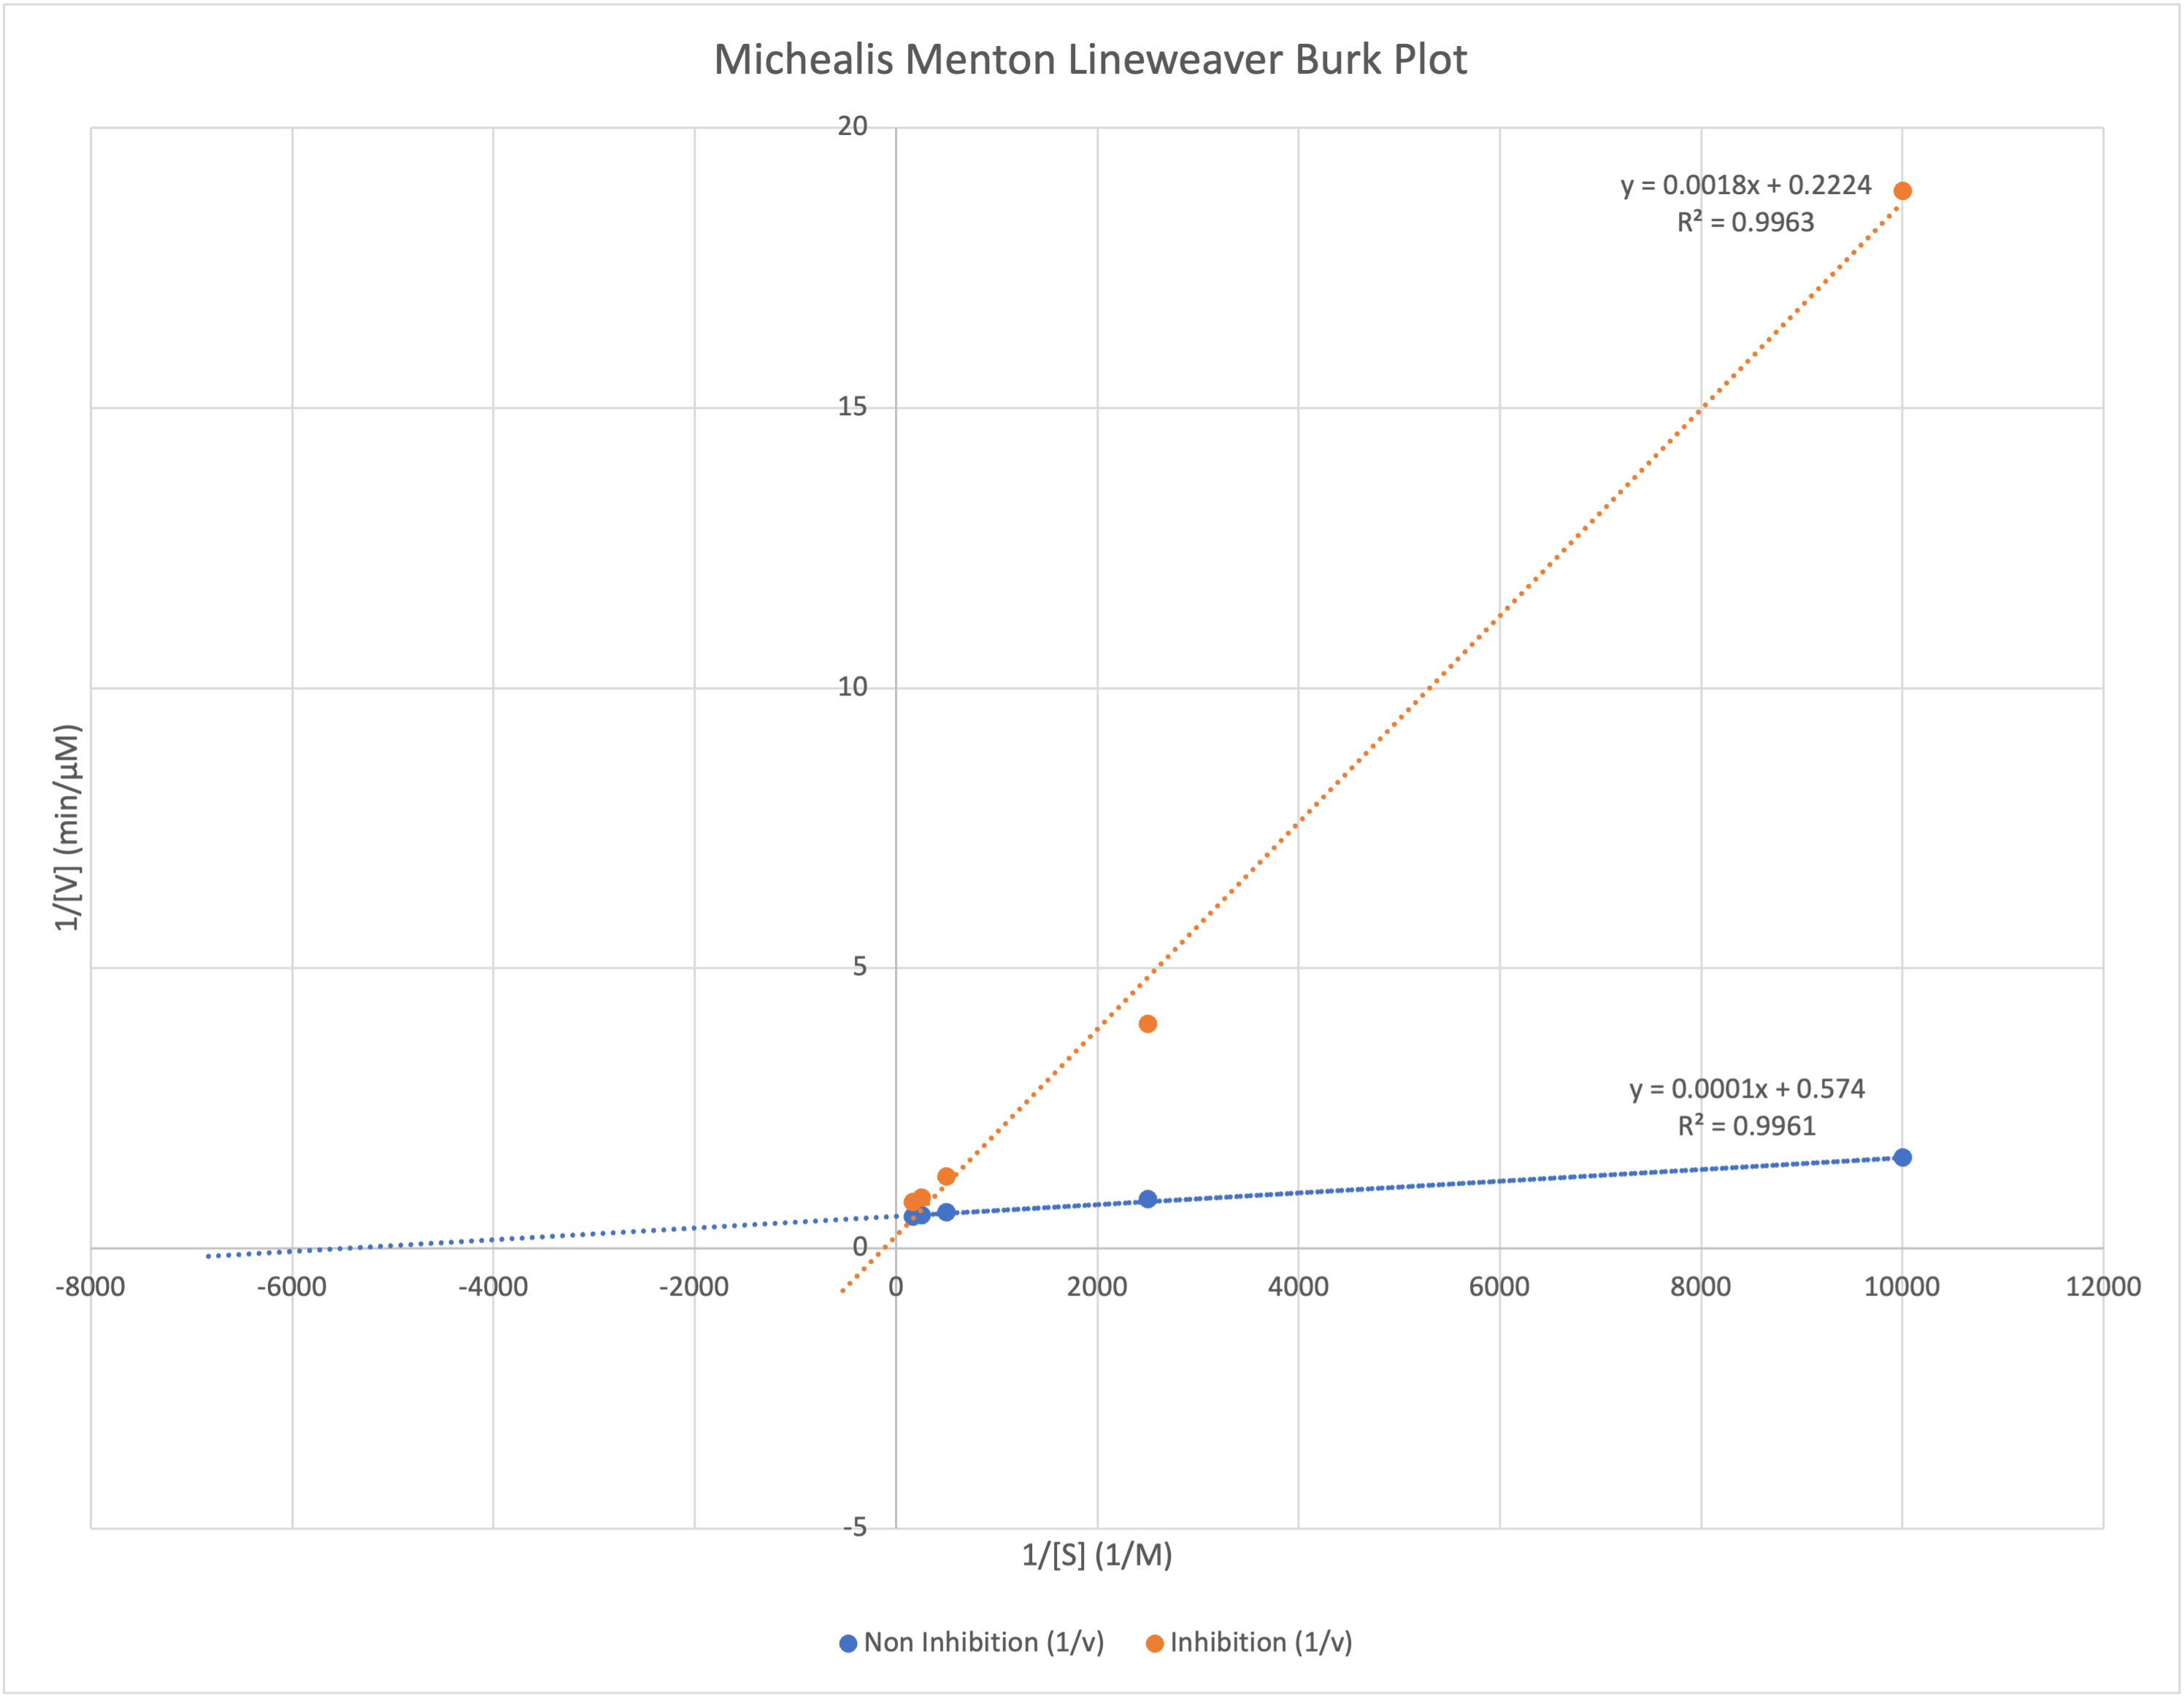
\includegraphics[width=0.8\textwidth]{photos/lbp.png}
  \caption{Lineweaver Burk plot of Substrate concentration (M) vs Velocity of Rection  ($\mu$M/min). }\label{fig3}
\end{figure}

In the Lineweaver-Burk plot, there is a noticeable difference in the
y-intercept values of both curves (0.2224 vs. 0.574) suggesting that the line
of best fit for the Lineweaver-Burk plot has a lesser fit than the Michaelis
Menton plot and thus is less accurate in this context. Moreover, in the
Michaelis Menton plot, the y-intercepts were almost similar (1.725 vs 1.789)
which should ideally be the case as 1/{V\textsubscript{max}} of both the curves
(inhibition vs. non-inhibition) should be equal.

Since we already have the two K\textsubscript{m} values, we only need to
calculate the two K\textsubscript{i} values which we can obtain using the
following equation:

\[\alpha = 1 + \frac{[I]}{K_i}\]
Where,

\[\alpha = \frac{K_m'}{K_m}\]
Where the $K_m'$ is the value of the Michaelis constant of the inhibitor
reaction and $K_m$ is the value at the non-inhibitor reaction. By plugging,

\[K_m' = 0.00237, K_m = 0.000211 \Rightarrow \alpha = 11.23\]

We know that 1\,mL of 0.033\,M of KH$_2$PO$_4$ was added to 10\,mL of citrate
buffer to make 11\,mL of solution. The resulting concentration of Potassium
Phosphate ([I]) = 0.003\,M.

Since we know [I], and $\alpha$, we can solve for the equation to obtain $K_i$:

\[K_i = \frac{[I]}{\alpha - 1}\]
\[K_i = \frac{0.003}{11.23 - 1} = 0.000293\,\text{M}\]

\subsection{Effect of Temperature on Enzymatic Activity}
The Arrhenius equation is used to relate the first-order rate constant for a
reaction (k) to the activation energy (Ea) for a chemical reaction.

\[k = Ae^{-Ea/RT}\]
After taking the natural log of both sides, we have:

\[ln(k) = ln(A) - (Ea/R).(1/T)\]
Where, y = \(ln(k)\); x = \((1/T)\); slope (m) = \(-(Ea/R)\); and y-intercept
(b) = \(ln(A)\). To obtain V\textsubscript{max}, the following equation can be
used: V\textsubscript{max} = k\textsubscript{cat}[E]\textsubscript{T}. We have,

$\Rightarrow$ Molecular weight of enzyme: 150,000\,g/mol.

$\Rightarrow$ Concentration of Enzyme (mg/L): 24.5\,mg/L.

$\Rightarrow$ Concentration of Enzyme (mol/L): $24.5 \times 10^{-3}/150,000$\,mol/L = $1.63 \times 10^{-7}$\,M = 0.163\,\mu\text{M}
\begin{table}[h]
  \begin{center}
    \begin{minipage}{300pt}
      \caption{Enzyme Activity at different Temperatures}\label{tab1}
      \begin{tabular}{  m{4em}  m{4em} m{4.5em}  m{4.5em}  m{4.5em} m{4.5em}}
        % {@{\extracolsep{\fill}}lcccccc@{\extracolsep{\fill}}}
        \toprule
        Temp. (K) & Absorbance with Enzyme (OD) & Absorbance without Enzyme (OD) & Absorbance adjusted\footnotemark[1] (OD) & Velocity ($\mu$M/s) & $K_{\text{cat}}$ (s$^{-1}$) \\
        \midrule
        288       & 0.110                       & 0.010                          & 0.100                                    & 0.57                & 3.49                        \\
        293       & 0.170                       & 0.012                          & 0.158                                    & 0.91                & 5.58                        \\
        298       & 0.190                       & 0.006                          & 0.184                                    & 1.06                & 6.50                        \\
        303       & 0.388                       & 0.016                          & 0.372                                    & 2.16                & 13.2                        \\
        308       & 0.576                       & 0.014                          & 0.562                                    & 3.27                & 20.0                        \\
        313       & 0.690                       & 0.028                          & 0.662                                    & 3.86                & 23.6                        \\\\
        \botrule
      \end{tabular}
    \end{minipage}
  \end{center}
\end{table}

We can then plot ln(K\textsubscript{cat}) vs 1/T to obtain the slope and
intercept of the Arrhenius equation. To ensure we don't get very small values
in the graph, the value of 1/T was multiplied by 1000 to obtain the following
graph.

\begin{figure}[h]
  \centering
  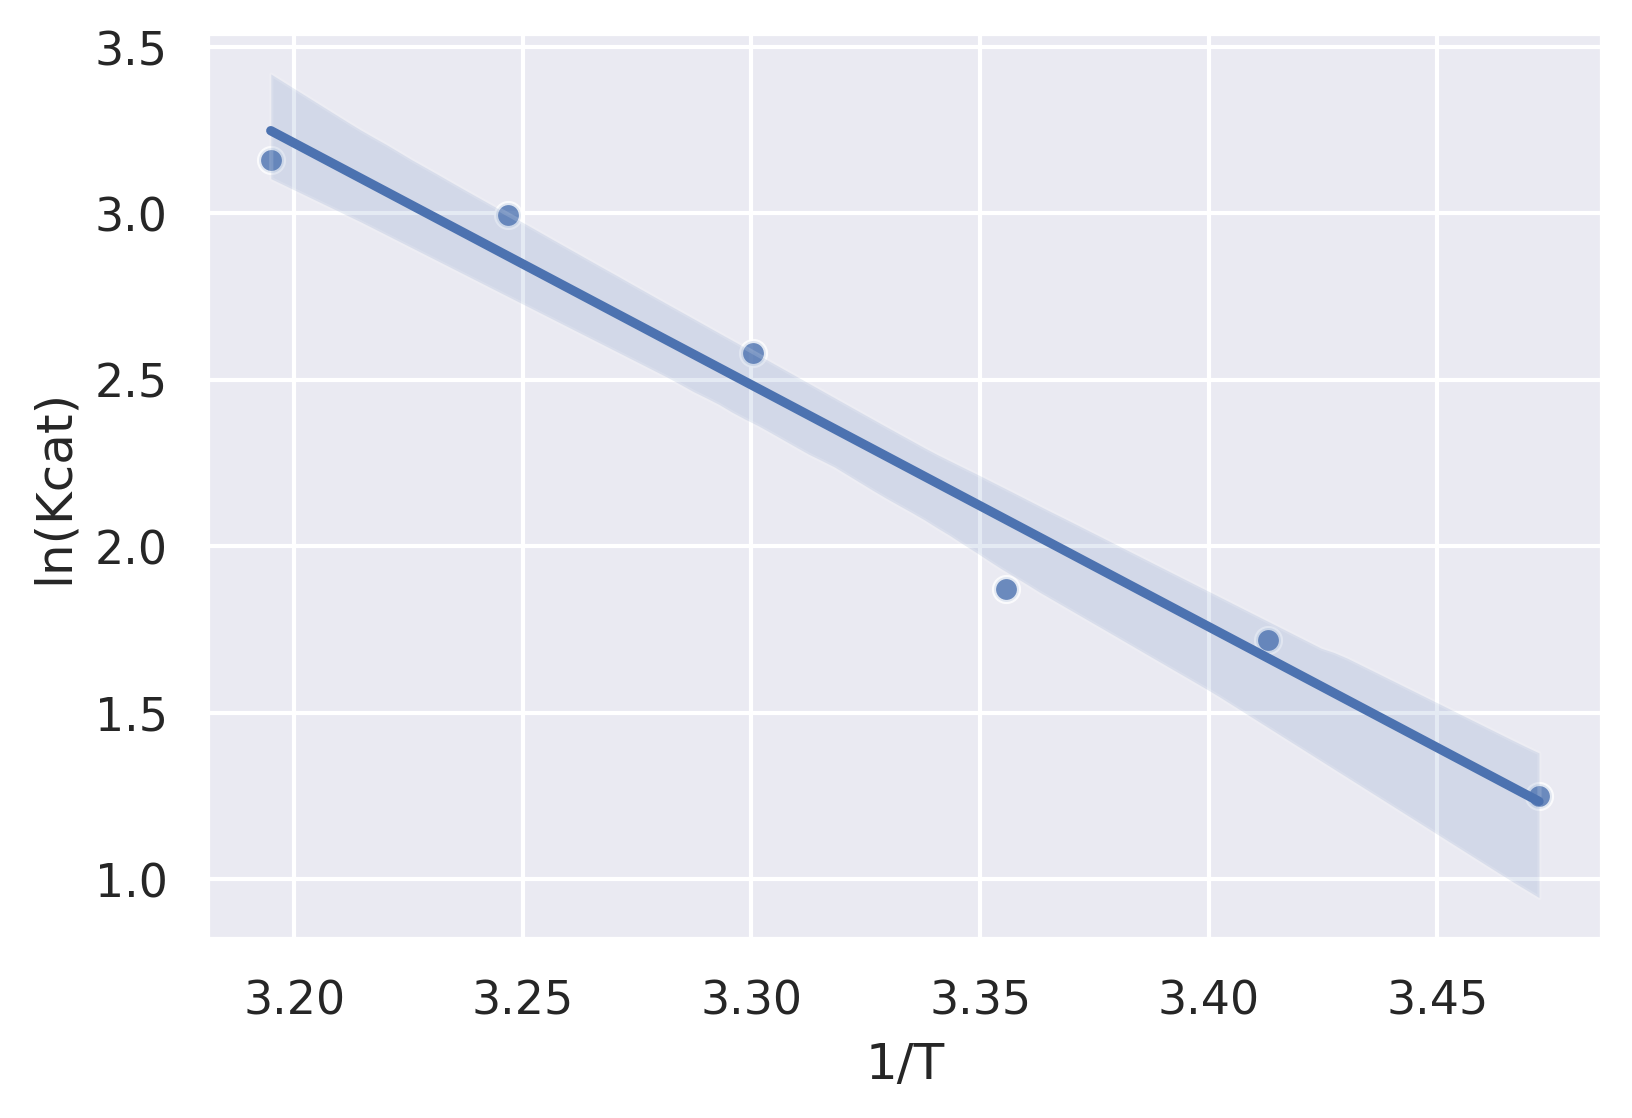
\includegraphics[width=0.8\textwidth]{photos/ln_graph.png}
  \caption{The plot of $\ln(k_{\text{cat}})$ (s$^{-1}$) vs. $1/T$ (K$^{-1}$)}\label{fig3_}
\end{figure}

To obtain slope and intercept, algebraically, two points were taken and the
equation was solved for two variables. The following equation of line was
obtained:

\[y = -7235x + 26.355\]
Where,

\[\text{slope} = -7235; \text{intercept} = 26.355\]
We know that $\text{slope} = -\frac{E_a}{R}$ and $\text{Intercept} = \ln(A)$;
Plugging, the values of $R = 8.314$\,J\,K$^{-1}$\,mol$^{-1}$ and slope =
$-7.235$,

\[E_a = -(-7235 \times 8.314) = 6.01 \times 10^4\,\text{J/mol}\]
Similarly,

\[\ln(A) = 26.355\]

\[A = 2.71 \times 10^{11}\,\text{s}^{-1}\]

\subsection{Sources of Error}\label{subsec2}
\begin{enumerate}
  \item One of the most prominent sources of error is the inaccuracy of measurement of
        time of incubation to calculate the velocity of the reaction.
  \item Followingly, due to fewer observations, the calibration curve obtained might
        not be perfect.
  \item Similarly, due to fewer data points, generating a line or curve of best fit
        could be difficult.
\end{enumerate}

\end{document}
